\section{CCWZ construction}
\label{seciton:ccwz construction}

As Goldstone bosons are massless, they play a crucial role in the low-energy dynamics.
To best describe this limit, we seek a parametrization of the fields in which they are the degrees of freedom.
This can be done using the CCWZ construction, named after Callan, Coleman, Wess, and Zumino.
As well as the original papers~\cite{Structure_of_phen_1,Structure_of_phen_2}, this section is based on~\cite{weinberg_1996_vol2,The_composite_NG_Higgs,effective_FT_with_NG_modes,morrison:ccwz_presentation}.


We saw that the Goldstone bosons correspond to excitations within the vacuum manifold.
The vacuum manifold corresponds to points in field space $\varphi$ that can be reached from the vacuum $\varphi_0$ with a transformation $g \in G$.
This means that we can write such excitations as
\begin{equation}
    \varphi = \tilde\Sigma \varphi_0, \quad \tilde \Sigma = \tilde \Sigma(\eta) = \exp{i \eta_\alpha T_\alpha}
\end{equation}
$\tilde \Sigma$ is thus a function from the parameter space, $\eta_\alpha \in \R^n$, to $G$,
\begin{align}
    \tilde \Sigma: \R^n \longmapsto G.
\end{align}
We then get space-time-dependent field configurations by making the parameters dependent on space-time.
We will for now assume $\eta_\alpha$ is constant.
This parametrization is highly redundant.
There are $n = \dim G$ parameters $\eta_\alpha$, but Goldstone's theorem says that there is one massless mode per broken generator.
Two elements $\tilde\Sigma$ and $\tilde\Sigma'$, related by
\begin{equation}
    \tilde \Sigma' = \tilde\Sigma e^{i \theta_a t_a}
\end{equation}
results in the same $\varphi$.
This is because  $e^{i \theta_a t_a} = h \in H$, and $h \varphi_0 = \varphi_0$, by assumption.
The set of all equivalent $\tilde \Sigma$'s is exactly the left coset, $gH = \setbuilder{gh}{ h \in H}$.
The set of cosets forms a new manifold, $G / H$, called the Goldstone manifold.
This is a manifold of dimension $\dim(G/H) = \dim(G) - \dim(H)$, which is the number of broken generators and thus also the number of Goldstone modes.
Membership of a certain coset form an equivalence relation, $g \sim g'$ if $g' = gh$.
This means that the cosets $gH$ form a partition of $G$ and that each element $g \in G$ belongs to one, and only one, coset.
To remove the redundancy in the parametrization, we need to choose one representative element from each coset.

By the inverse function theorem, any mapping between manifolds $f: \Em \mapsto \mathcal{N}$ that has a non-degenerate differential, that is an invertible Jacobian, at a point $p \in \Em$, is invertible in a neighborhood of $p$.
The map
\begin{equation}
    \tilde \Sigma(\xi, \theta) = \exp{i \xi_i x_i} \exp{i \theta_a t_a}
\end{equation}
is invertible at $p = (\xi_i = 0, \theta_a = 0)$, which is mapped to the identity, as the Jacobian is the identity matrix.
This means that, in a neighborhood $U \subset G$ of the identity, each element $g$ has a unique representation $g = \Sigma$~\cite{smooth_manifolds}.
Furthermore, two elements $\tilde \Sigma'$ and $\tilde \Sigma$ related by $\tilde \Sigma' = \tilde \Sigma h$, $h \in H$ have the same $\xi$-arguments.
We see that $\xi_i$ parametrize $G/H$, in the neighborhood of the identity.
We therefore demand that $\tilde \Sigma$ always appear in the standard form
\begin{equation}
    \Sigma(\xi) = \tilde \Sigma(\xi, 0) = \exp{i \xi_i x_i}.
\end{equation}
The field $\varphi(x)$ can therefore be written as
\begin{equation}
    \varphi(x) = \Sigma(x) \varphi_0 = \exp{i \xi_i(x) x_i} \varphi_0,
\end{equation}
and $\xi_i(x)$ can be associated with the Goldstone bosons.

In the linear sigma model, the original $\Olie(N)$ symmetry is broken down to $\Olie(N-1)$, which transforms the remaining $N-1$ fields with vanishing expectation values into each other.
However, $\Olie(N)$ consists of two disconnected subsets, those matrices with determinant 1 and those with determinant -1.
There is no continuous path that takes an element of $\Olie(N)$ with determinant of $-1$ to an element with determinant 1.\footnote{A simple proof of this is the fact that the determinant is a continuous function, while any path $\det M(t)$ such that $\det M(1) = -1,\, \det M(0) = 1$ must make a discontinuous jump.}
The set of symmetries that are connected to the identity is
\begin{eqnarray}
    G = SO(N) = \setbuilder{M \in \Olie(N)}{ \det M = 1}.
\end{eqnarray}
If we choose $\varphi_0 = (0, 0, ..., v)$, then it is apparent that the ground state is invariant under the rotations of the $N-1$ first fields, so the unbroken symmetry is  $H = \SO(N-1)$.
The Goldstone manifold is $G/H = \SO(N) / \SO(N-1)$.

Consider the case of $N = 3$, which is illustrated in \autoref{fig:ground state manifold}.
$G$ is the rotations of the sphere, while $H$ is rotations around $\varphi_0$, $\SO(2)$.
The Goldstone manifold consists of the rotations of $\varphi_0$ to other points of the sphere, i.e. $G/H = \SO(3)/\SO(2) = S^2$, the 2-sphere.
This is not a Lie group, as translating $\varphi$ in a closed path around the sphere may result in a rotation around the z-axis.
This is illustrated in \autoref{fig:Curvature of SO(3)}


To check that $\xi_i$, in fact, are the Goldstone modes, we study the way they appear in the Lagrangian.
As they are massless, no mass term of the form $M_{ij} \xi_i \xi_j$ should appear.
The original Lagrangian $\Ell[\varphi]$ was invariant under global transformations $\varphi(x) \mapsto g \varphi(x)$.
However, any terms that only depend on $\varphi(x)$, and not its derivatives, will also be invariant under a \emph{local} transformation, $\varphi(x) \mapsto g(x)\varphi(x)$.
Our parametrization of the fields, $\varphi(x) = \Sigma(x)\varphi_0$ is exactly such a transformation, which means that any such terms are independent of the Goldstone bosons.
We can therefore write
\begin{equation}
    \Ell[\varphi] = \Ell_{\mathrm{kin}}[\varphi] + V(\varphi_0),
\end{equation}
where all terms in $\Ell_{\mathrm{kin}}$ are proportional to at least one derivative term, $\partial_\mu \varphi(x)$.
Inserting the parametrization into this derivative term, we get
\begin{equation}
    \partial_\mu \varphi(x) = \partial_\mu [\Sigma(x) \varphi_0]
    = \Sigma(x) [\Sigma(x)^{-1} \partial_{\mu} \Sigma(x)] \varphi_0.
\end{equation}
The Lagrangian will therefore depend on $\xi_i$ via terms of the form $\Sigma(x)^{-1}\partial_\mu \Sigma(x)$, which is called the Mauer-Cartan form.
This is a $\mathfrak g$-valued function, which means that it can be written as
\begin{align}
    i\Sigma(x)^{-1}\partial_\mu \Sigma(x) & 
    = d_{\mu}(x) + e_{\mu}(x), \\
    d_{\mu} & = i x_i d_{ij}(\xi) \partial_\mu \xi_j, \\
    e_{\mu} & = i t_a e_{ai}(\xi)\partial_\mu \xi_i,
\end{align}
where $d_{ij}$ and $e_{ai}$ are as-of-yet unknown real valued functions of $\xi$~\cite{weinberg_1996_vol2,Watanabe:effective_lagrangian}.

\subsection*{Transformation properties of Goldstone bosons}
We can deduce how the Goldstone bosons transforms under $G$ from how $\varphi$ transforms.
In general, 
\begin{equation}
    \varphi' = g \varphi = (g \Sigma(\xi)) \varphi_0 = \Sigma(\xi') \varphi_0 \quad g \in G.
\end{equation}
While $\Sigma(\xi')$ has the standard form by assumption,
\begin{equation}
    \Sigma(\xi') = \exp{i \xi'_i x_i},
\end{equation}
$g\Sigma(\xi)$ does not, in general.

\begin{figure}[h]
    \centering
    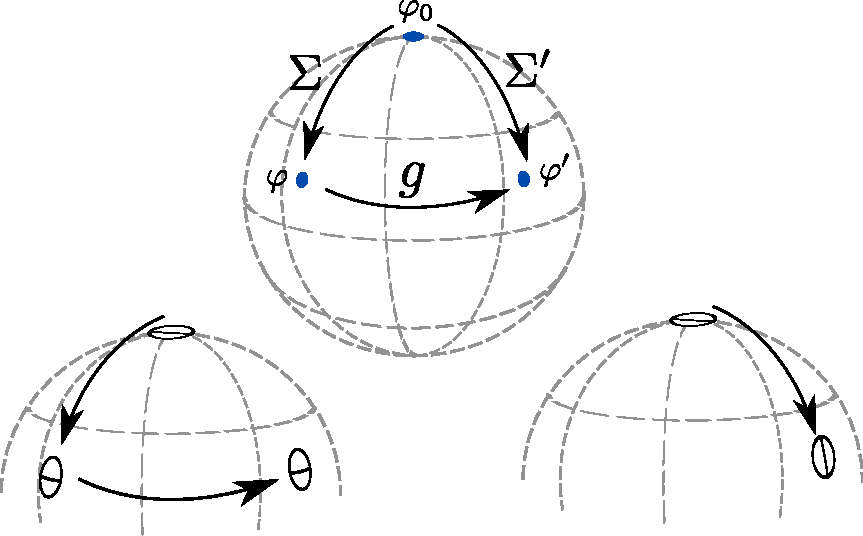
\includegraphics[width=0.8\textwidth]{figurer/curvature.pdf}
    \caption{The top figure illustrates the transformation of $\varphi_0$ to $\varphi$ and then $\varphi$, and the alternative transformation $\varphi_0 \rightarrow \varphi'$. The bottom figure illustrates how this can rotate a neighborhood of $\varphi_0$ differently.}
    \label{fig:Curvature of SO(3)}
\end{figure}
\autoref{fig:Curvature of SO(3)} illustrates this in the case of $G = \SO(3)$.
$\Sigma(\xi)$ transforms $\varphi_0$ to $\varphi$, then $g$ transforms $\varphi$ to $\varphi' = \Sigma(\xi') \varphi_0$.
Assuming $\varphi$ and $\varphi'$ are close enough to $\varphi_0$, we can write $\Sigma(\xi)$ and $\Sigma(\xi')$ on the standard form.
However, if we follow a small neighborhood around $\varphi_0$ as it is acted on by $\Sigma(\xi)$, then $g$, it will be rotated by the time it arrives at $\varphi'$ when compared to the same neighborhood if it was acted on by $\Sigma(\xi')$.

$g\Sigma(\xi)$ and $\Sigma(\xi')$ are in the same coset, as they by assumption corresponds to the same physical state.
This means that we can write $g\Sigma(\xi) = \Sigma(\xi') h(g, \xi)$, where $h(g, \xi) \in H$.
The transformation rule of $\xi$ under $G$ is therefore implicitly defined by
\begin{equation}
    \Sigma(\xi') = g \Sigma(\xi) [h(g, \xi)]^{-1}.
\end{equation}
This is, in general, not a linear representation, which is why this construction also is called a \emph{non-linear realization}.
Using the transformation rule, we can obtain the transformation rule of the Maurer-Cartan form.
We use the shorthand $\Sigma = \Sigma(\xi),\, \Sigma' = \Sigma(\xi')$, and $h = h(g, \xi)$.
This gives
\begin{align*}
    \Sigma^{-1} \partial_\mu \Sigma
    \rightarrow 
    & \, \Sigma'^{-1} \partial_\mu \Sigma' \\
    & = (g \Sigma h^{-1})^{-1} \partial_\mu (g \Sigma h^{-1}) \\
    & = (h \Sigma^{-1} g^{-1}) g [(\partial_\mu \Sigma)h^{-1} + \Sigma \partial_\mu h^{-1}] \\
    & = h \Sigma^{-1} (\partial_\mu \Sigma) h^{-1}
    + h \partial_\mu h^{-1} \\
    & = h (\Sigma^{-1} \partial_\mu \Sigma + \partial_\mu) h^{-1}.
\end{align*}
In terms of $d_\mu$ and $e_\mu$,
\begin{align}
    d_\mu & \rightarrow h d_\mu h^{-1} \\
    e_\mu & \rightarrow h (e_\mu + i\partial_\mu )h^{-1}.
\end{align}
These are our building blocks for constructing a general, $G$-invariant effective Lagrangian.
The trace of a product of $d_\mu$'s are invariant under $G$,
\begin{equation}
    \Tr{d_\mu d_\nu \dots d_\rho} 
    \rightarrow
    \Tr{h d_\mu h^{-1} h d_\nu h^{-1} h \dots d_\rho h^{-1}}
    = \Tr{d_\mu d_\nu \dots d_\rho},
\end{equation}
where we have used the cyclic property of trace.
However, the terms must also obey the other symmetries of the Lagrangian, such as C or P-parity and Lorentz invariance.
The last criterion excludes any terms with free spacetime indices.
In \autoref{section:chiral pertubation theory}, we will construct an effective Lagrangian in powers of $d$.
The lowest order terms are therefore
\begin{equation}
    \label{first order terms CCWZ}
    \Tr{d_\mu} \Tr{d^\mu}, 
    \quad 
    \Tr{d_\mu d^\mu}.
\end{equation}
We see that $e_\mu$ transforms like a gauge field, with the gauge group $H$.
If we include massive degrees of freedom and not only the Goldtone modes, $e_\mu$ is used to create a covariant derivative of the massive modes.
We are only interested in the Goldstone modes and will therefore be satisfied with $d_\mu$.
With these tools, we can create an effective theory of quantum chromodynamics at low energies.

